\chapter{Methodology \& Model design}
\label{chap:methodology}

\section{Programming Language}
\label{sec:language}

Given the computational nature of the orbit determination problem introduced in \Cref{chap:introduction}, a decision for the appropriate programming language in which the model will be developed has to be made. In today's academic environment, several scientists chose to develop their code in dynamic languages such as MATLAB or Python, which enhance productivity by giving a variety of tools to developers. However, these dynamic programming languages suffer during problems which can be classified as computationally intensive, leading to the use of languages such as C or Fortran when dealing computationally heavy problems \cite{Julia-2017}. 

The problem with the latter languages is that they do not offer the productivity provided by the dynamic languages, which have arguably made the development of scientific code fairly easier, leading to developers having to perform a trade-off for each problem to choose the appropriate language.  This problem is frequently described as the two language problem in literature. A solution which combines both the productivity and performance and thus solves the two language problem is Julia \cite{Julia-2017}. From \Cref{fig:julia_bench}, it can be concluded that code written in Julia will achieve similar benchmark times to C \cite{julia-benchmark}, while also providing the user with high level functions and options to write code in a more productive manner.

\begin{figure}[h]
	\centering
	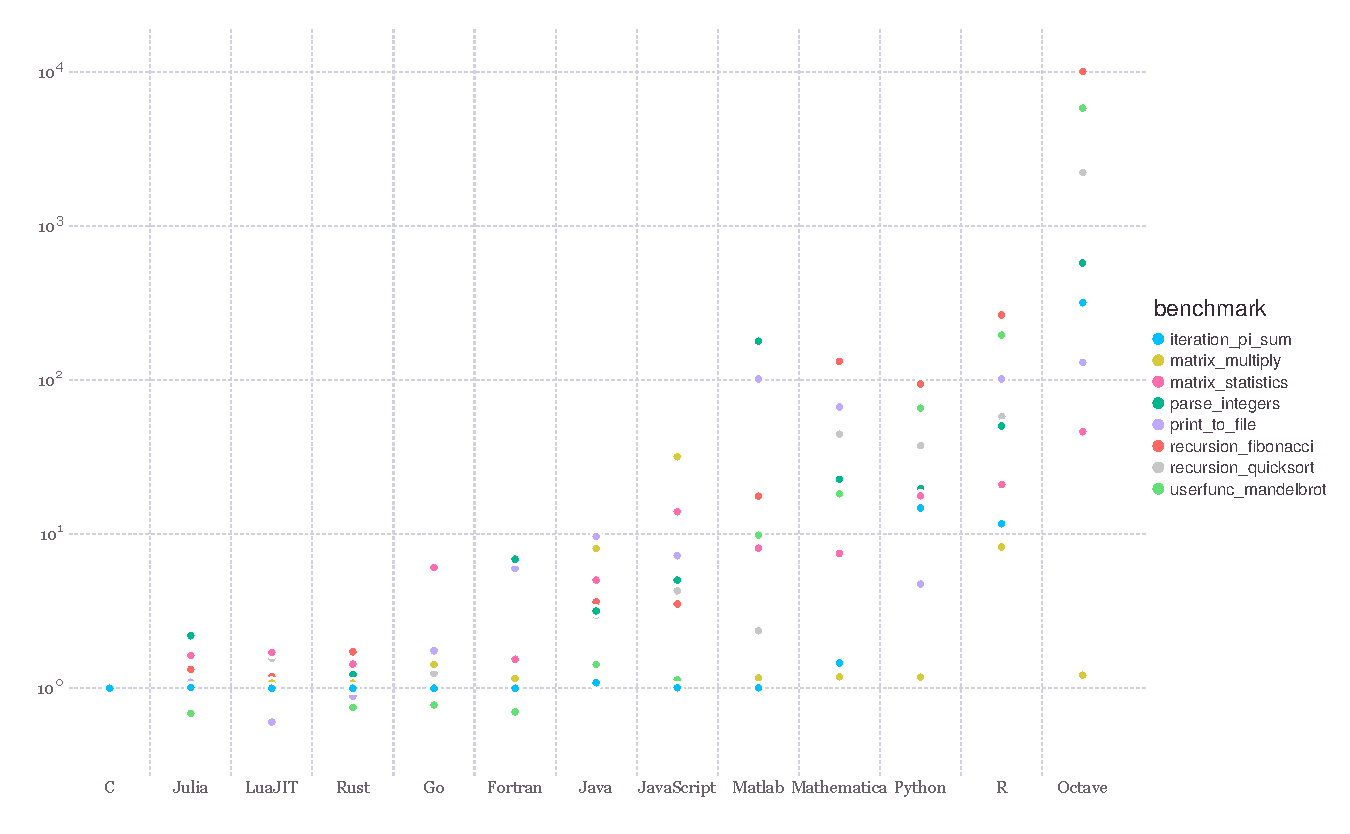
\includegraphics[width=\textwidth]{Figures/Chapter2/julia_benchmarks.pdf}
	\caption{Normalized benchmark time of some problems against the C implementation for different programming languages \cite{julia-benchmark}}
	\label{fig:julia_bench}
\end{figure}

In the context of this thesis, it can be expected that the code developed will be computationally intensive, given the fact that numerical integrators used to perform the propagation of the asteroids for the fitting procedure (which will undoubtedly run several times until a solution is identified), leading to a need for performance. In addition, coordinate transformations, missing objects from the images generated and other pitfalls require a productive way to deal with these problems. Since the two language problem is being faced, the decision has been made early to use Julia as the programming language for the development of this thesis.




\section{Orbital Dynamics}

For the description of the orbit determination problem being faced from the perspective of astrodynamics, we can simplify the problem into two separate problems, namely:

\begin{enumerate}
	\item The orbit followed by the Hera spacecraft during the observation period.
	\item The behavior of the two asteroids Didymos \& Dimorphos.
\end{enumerate}

Once an adequate description for both of these sub-problems has been given, they can then combine them into a single dynamics model using the appropriate reference frames and transformations between them. After this combination is complete, the image generation procedure can be built and different types of errors can be added.  
   